%!TEX root = ../thesis.tex
%*******************************************************************************
%****************************** Third Chapter **********************************
%*******************************************************************************

\chapter{Subsampling and Nested Sampling}\label{ch:chapter3}

% **************************** Define Graphics Path **************************
\ifpdf
    \graphicspath{{Chapter3/Figs/Raster/}{Chapter3/Figs/PDF/}{Chapter3/Figs/}}
\else
    \graphicspath{{Chapter3/Figs/Vector/}{Chapter3/Figs/}}
\fi

\section{Non-Deterministic Likelihoods in Nested Sampling}

In cosmology, particle physics, machine learning and numerical sciences in general we often find that the size of the available data far exceeds our computational capabilities to  analyse the full dataset in its raw form. In such cases typically there are several compression steps which are applied to the data (such as averaging \& binning). To discuss the solution considered in this chapter, we must first introduce the concept of `subsampling' data to generate an approximate likelihood. `Subsampling' in the context of this thesis refers to randomly selecting a subset of the full set of data points to generate the likelihood function. However, the subsample is only an approximation to the full information encoded in the whole dataset. Additionally, subsampling is non-deterministic because the subsamples are random and produce different results than the full dataset would. 

Consider that there are $n=100$ data points but we are restricted to only sample, say, a randomly selected subsample of $m=10$ points at each step. Then, we must contend with the fact that, depending on our luck, the very same set of parameters, $\theta$, may sometimes be acceptable or unacceptable in the nested sampling acceptance criteria $L(\theta)>L_i$(refer back to \cref{section:NSmath} for a recapitulation)--owing to the error on the likelihood introduced from having to subsample. This means that the likelihood is non-deterministic because the subsample changes at every likelihood evaluation. This also renders unusable the two mainstream-adopted nested sampling packages--\texttt{MultiNest}~\cite{Feroz_2009} and \texttt{\texttt{PolyChord}}~\cite{Handley_2015}--because they fail to converge due to their non-compatibility with non-deterministic likelihoods(this will be discussed further in \cref{sec:nondet}). One may suggest that this turmoil of non-determinism may be avoided by simply always using the same subset of $m=10$ data points--utilising deterministic subsampling--as this would allow all the algorithms that we built for deterministic data to still be viable. The issue is that this would result in much more biased data and therefore biased results. Using new subsets of the data at each sample, we get a picture of the information encoded across the whole dataspace rather than a localised version of it. Over multiple samples one can get a sufficiently accurate picture of the greater landscape of the likelihood manifold being explored. This is why we shall explore ways to make non-deterministic likelihoods more compatible with nested sampling--at least to the extent where nested sampling actually converges. We cover this in \cref{sec:nondet}, which comes after the next \cref{sec:control_variates}, where we introduce an efficient and accurate method to extract information spanning the whole dataspace. The method does this while reducing computational costs by not having to explicitly sample the whole dataspace. This is performed by the use of control variates, a variance reduction tool for Monte Carlo methods. This efficient subsampling method was first introduced in rigorous mathematical form by Quiroz et al.~\cite{Quiroz_2018}. Our first contribution is in the translation of this efficient data subsampling method into an easily digestible format for researchers from a physics or engineering background. We find that this result has potentially wide applicability in astrophysics and cosmology. Thus, it is pertinent for this work to be reiterated in an accessible format for physicists as we do in the next section.


\section{Control Variate Subsampling for Physicists and Engineers}\label{sec:control_variates}

In this section we shall introduce an efficient and accurate subsampling method that uses control variates to reduce subsampling induced variance. They leverage the error information on known quantities to reduce the error on unknown quantities. The control variates leverage the principle of locality in data. That is, that nearby data points result in similar likelihoods. The idea behind control variates is that data can be clustered and averaged. This is due to the continuity of the log-likelihood as a function of the data coordinates, nearby data points are likely to have similar characteristics. In other words, whichever function uses these data points as parameters has to be continuous if it is physical thus there are definite effects of locality, which can be taken advantage of through Taylor expansions. Throughout this introduction we shall explicitly demonstrate the method for a 2-dimensional example case--for the ease of comprehension of the reader. In practice, this is sufficient for astronomical examples which consider the two-dimensional sky. However, the method is easily generalised to higher dimensions.

Consider a set of data, $\{ x,y \}= \{ \{x_1,x_2,...,x_n\}, \{y_1,y_2,...,y_n\} \}$, and a hypothesised physical model, $y= f(x,\theta)$. The $\theta$ are the parameters of the proposed model, where log-likelihood of observing the whole dataset, $\{x_1,x_2,...,x_n,y_1,y_2,...,y_n\}$, can be written out as
\begin{equation}
\log L = \sum_{i=1}^{n} l (\textbf{z}_{i},\theta).
\end{equation}
%
Here the $l (\textbf{z}_{i},\theta)$ are the log-likelihood contributions of the $i$th data points, represented in vectorised format, $\textbf{z}_{i}= \{x_i,y_i\}$. This likelihood is only applicable for independent and identically distributed data, i.e. the uncorrelated case. In practice, we may encounter datasets with $n$ large enough to where evaluating this sum repeatedly can become computationally intractable. One may initially think to approximate the whole sum through simple random sampling (SRS),
%
\begin{equation}
\log \hat{L} = \frac{n}{m} \sum_{i=1}^{m} l ( \textbf{z}_{u_{i}},\theta).
\label{eq:fgf}
\end{equation}
%
Where $u_i$ are a random set of integers between one and $n$ such that we have the randomly selected subset of the dataset $\{ z_{u_{i}} \} \subset \{\{x_1,y_1\},\{x_2,y_2\}...,\{x_n,y_n\}\}$.  We have scaled up the log-likelihood of the subsample above with the $\frac{n}{m}$ factor--assuming that the subsample of $m$ terms is randomly sampled from the full dataset without bias and is large enough to be sufficiently representative of the information contained within the whole dataset. If the error associated with each of the log-likelihood contributions is $\sigma$, then total standard deviation of the SRS subset of $m$ elements, $\sigma_m$, scales up as
%
\begin{equation}
\sigma_m = \sqrt{\frac{n}{m}} \sigma_{n}.
\end{equation}
%
Here $\sigma_{n}$ is the original standard deviation of the full set. In general, the standard deviation would increase with $O(\sqrt{\frac{n}{m}})$. This is undesirable since the point of subsampling is that we want $m \ll n$. In the case of the Gaia dataset of $340$ billion celestial measurements~\cite{2016,https://doi.org/10.48550/arxiv.2208.00211} we may often choose a subset of $10$ million stars, leaving us with a roughly $100$-fold increase in log-likelihood standard deviation utilising the simple random sampling method. Now that we have introduced SRS and its perils, we shall introduce control variate subsampling.

\subsubsection{Using Control Variates to Reduce Variance of Simple Random Sampling}

We shall refer to the efficient control variates as $\bar{l}_i$. Initially, we pre-select $K$ points in data-space and label them `cluster centres'. The control variates are merely second order Taylor expansions around the nearest cluster centre in data-space. We start by cycling through all our $n$ data-points to classify their respective clusters to which they are closest to. Then, we Taylor expand the log-likelihood contributions of each data point, $\textbf{z}_i$, around their respective cluster centre, $\bar{\textbf{z}}_{k_{i}}$. The $k_{i}$ labels the cluster centre which the data point labelled by $i$ belongs to. The Taylor expansion is of the form:
%
\begin{equation}
\begin{aligned}
\bar{l}(\textbf{z}_i,\theta) = l(\bar{\textbf{z}}_{k_{i}},\theta)+ \nabla_z l(\bar{\textbf{z}}_{k_{i}},\theta) \cdot (\textbf{z}_i-\bar{\textbf{z}}_{k_{i}})+ \\ 
\frac{1}{2}(\textbf{z}_i-\bar{\textbf{z}}_{k_{i}})^\intercal  \nabla_z^\intercal \nabla_z l(\bar{\textbf{z}}_{k_{i}},\theta)(\textbf{z}_i-\bar{\textbf{z}}_{k_{i}}).
\end{aligned}
\label{eq:taylor}
\end{equation}
%
Where $\nabla_z$ is the gradient operator with respect to data-space. Thus, the second term includes a dot product and the third is a matrix product. This Taylor expansion above gives us the control variate for each point, $\bar{l}(\textbf{z}_i,\theta)$. The control variates express the information encoded in the global landscape of the log-likelihood over all of data-space for a computationally cheap cost. 
Utilising the above expression, control variate subsampling leverages such $\bar{l}(\textbf{z}_i,\theta)$ to approximate the full dataset sample in an efficient manner in the following way:
\begin{equation}
    \log \hat{L}= \sum_{i}^{n} \bar{l}(\textbf{z}_i,\theta) + \frac{n}{m} \sum_{i=1}^{m} \left[ l(\textbf{z}_{u_i},\theta) - \bar{l}(\textbf{z}_{u_i},\theta) \right].
\label{cvv}
\end{equation}
%
The above equation is an approximation to the log-likelihood through simple random subsampling with control variates added to reduce the variance. The terms in the above equation containing $\bar{l}$ make up the control variates, which work to reduce the variance on a random variable. Intuitively, the control variates encode information that spans the whole of dataspace through Taylor expansions around the cluster centres in dataspace. The special property of the control variates is that they are computationally cheap to evaluate. The larger our $K$ value, the fewer the subsamples, $m$, we need at each sample of the above function to provide equivalent accuracy. Furthermore, the larger the raw dataset size, $n$, the more we may increase $K$ to boost the accuracy of control variate subsampling. This means that control variate subsampling becomes more favourable over SRS as our raw dataset size increases. Increasing $K$ means that with minimal extra costs we can significantly improve the accuracy of our subsampling while maintaining the same subsample size, $m$. For further detail see \cref{sec:computational_costs}, ``Computational Costs''. We now move onto a concrete example for the newly introduced control variate subsampling to further build intuition.


\subsubsection{Concrete Example: Gaussian Likelihood}

In cosmology, we usually model the errors on the response variable, $y= f(x,\theta)$, as normally distributed. Thus the log-likelihood contribution of the observed data points $\{x_i,y_i \}$ should be of form
%
\begin{equation}
   l (\textbf{z}_{i},\theta) = - \log \sqrt{2\pi} \sigma_i -\frac{1}{2\sigma_i^2}(y_i-f(x_i, \theta))^2.
\end{equation}
%
Using this particular log-likelihood function, the terms in \cref{eq:taylor} would be written out explicitly as:
%
\begin{align}
   \nabla_z l(\bar{\textbf{z}}_{k_{i}},\theta) &= \frac{1}{\sigma_{k_{i}}^2} \begin{pmatrix}(y_{k_{i}}-f)f'\\-(y_{k_{i}}-f)\end{pmatrix},\\
   \nabla_z \nabla_z l(\bar{\textbf{z}}_{k_{i}},\theta) &=  \frac{1}{\sigma_{k_{i}}^2} \begin{bmatrix}
-f'^2+(y_{k_{i}}-f)f'' & f' \\
f' & -1 \\
\end{bmatrix}
\end{align}
%
For clarity, we have suppressed dependence on data and parameters in $f$, $f'$ and $f''$ in the above equations. To develop intuition, let us now explore the case where the proposed model describing the data is linear:
\begin{equation}
    f(x_i,\theta) = bx_i+ c.
\label{eq:strt}
\end{equation}
\begin{figure} 
\centering    
\includegraphics[width=1.0\textwidth]{Chapter3/Figs/Raster/fig3_27.pdf}
\caption{In this figure we have our randomly uniformly generated data points, $\textbf{z}_i= \{x_i,y_i \}$, plotted with the axes representing the $x$ and $y$ coordinates. The 5 red squares represent the cluster centres, according to which each data point is classified and then colour coded appropriately. For example, the turquoise colour coloured points are the ones closest to the cluster centre at $(0,1)$. Thus the Taylor approximation, \cref{eq:taylor}, for the turquoise points would be expanded around the $(0,1)$ cluster centre. The blue line through the centre of the points is the function $y=f(x,\theta)$. The $m$ subsamples, referred to in \cref{cvv}, would be some randomly chosen subsamples. These $m$ points are visualised by the points, among the $100$ data points, that are marked by the black crosses.}
\label{fig:one}
\end{figure}
Consider that we randomly generate $100$ uniformly distributed $x$-data points in the range $x=[-1,1]$ and simulate some Gaussian error in association to their corresponding $y$-values. Then we select $K=5$ equally spaced cluster centres on the line, $f(x_{i}, \theta )$. We classify each of our previously generated $100$ data points to their corresponding closest cluster centre. This process is visualised in \cref{fig:one}.


\begin{figure} 
\centering    
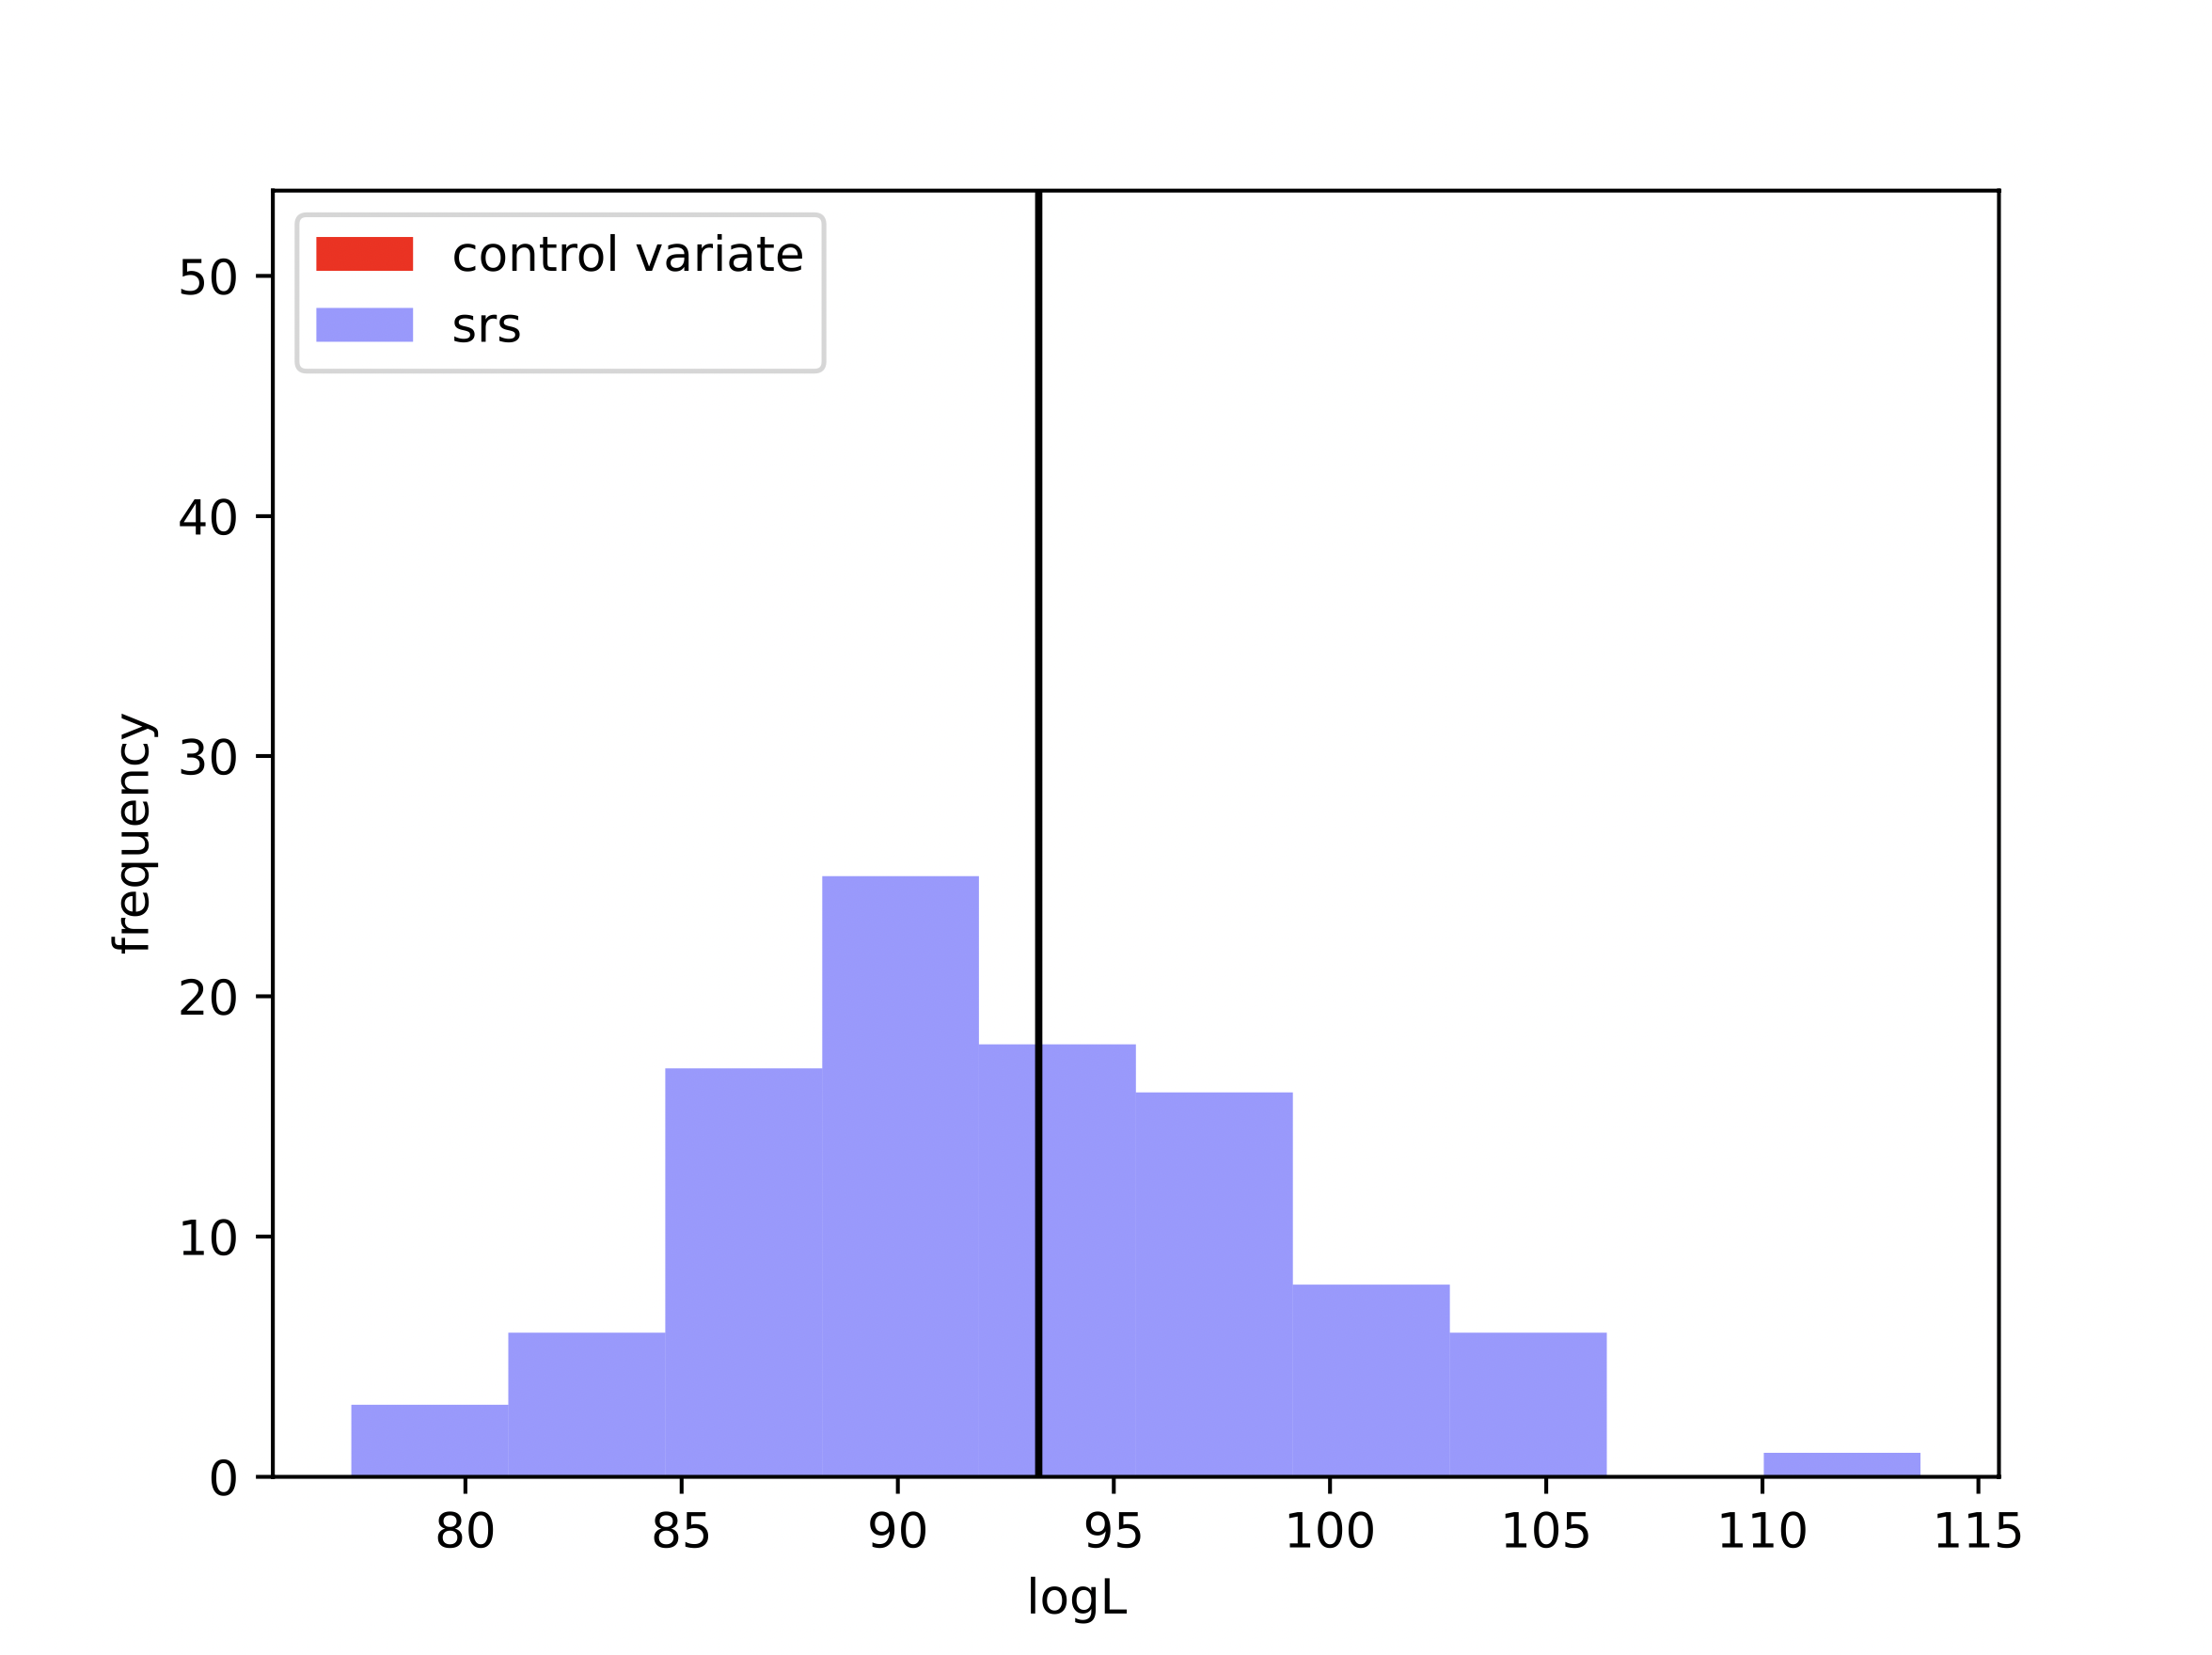
\includegraphics[width=1.0\textwidth]{Chapter3/Figs/regen3_28.png}
\caption{ The plotted histograms represent the total log-likelihood values for the linear $f(x,\theta)$ mentioned above in \cref{eq:strt}. There are 100 $\log L(\theta)$ samples plotted for both histogram plots. The $\theta$ chosen for these subsamples of $\log L(\theta)$ are the true values of the parameters of our model. These are namely $b=2$ and $c=1$, referring to \cref{eq:strt}. The black vertical line represents the true value of the total log-likelihood. The blue histogram represent the values estimated by the SRS method (without control variates). The values estimated by control variate subsampling are also plotted on the figure as red histograms but, as expected, they cannot be seen at the scale of this graph. This is because, beyond machine precision, there is no noise in the control variate subsampling log-likelihood values as the underlying function is linear. This is analogous to the mean and standard deviation being sufficient statistics to reconstruct a dataset.}
\label{fig:two}
\end{figure}

Having built an intuition regarding the meaning of the `hyperparameters'--$K$, $m$, and $n$--and their relation to the `model' and data, we move towards analysing the results produced by control variate subsampling as applied to this concrete example case of a Gaussian likelihood with a linear function as the `model'. Consider that we approximate the total log-likelihood with SRS, as in \cref{eq:fgf}. We set the number of subsampled points, $m$, to 55 and repeat this log-likelihood approximation $100$ times--each time choosing a different randomly selected subsample of 55 points from the $n=100$ total. Consider, that we also try to approximate the total log-likelihood with control variate subsampling, as in \cref{cvv}. We repeat this process 100 times as well. To maintain a like-for-like comparison, we try to keep the computational cost constant for both control variate subsampling and SRS. We can do this by choosing the following hyperparameters for the control variate subsampling case: number of clusters, $K=5$, and the number of subsamples, $m=20$. We go into further detail regarding the computational costs and how we arrive at these numbers in the \cref{sec:computational_costs} `Computational Costs'. The reader should keep in mind that this is the trivial case due to it being a linear function and the Taylor expansions in the control variates being second order. Thus the control variates subsampling ends up being analytically equal to the full raw dataset likelihood sample. We plot all these results as histograms in the \cref{fig:two}.


We now move onto a non-trivial case in order to show the effect of subsampling where
%
\begin{equation}
    f(x_i,\theta) = bx_i^3+ c.
\label{eq:tertiary poly}
\end{equation}
%
As emphasised before, there are several different moving parts to the control variate method, so we shall again try to build further intuition. We plot the function from \cref{eq:tertiary poly} in data-space in \cref{fig:three}, along with all the other `hyperparameters' of the method itself--$K$, $n$ and $m$. Such that everything is visualised . Note that for the purpose of the figure we give the following numerical values to the hyperparameters for less visual clutter: $K=5$, $n=100$, and $m=20$.
%
\begin{figure} 
\centering    
\includegraphics[width=1.0\textwidth]{Chapter3/Figs/Raster/fig3_30.pdf}
\caption{ This graph illustrates the control variate subsampling method described by \cref{cvv}--it aids the reader to better understand what the `hyperparameters', $K$, $m$, and $n$, mean. Our randomly uniformly generated data points $\textbf{z}_i= \{x_i,y_i \}$, plotted with the axes representing the $x$ and $y$ coordinates. The 5 red squares represent the cluster centres, according to which each point is classified and then colour coded appropriately. The blue line through the centre of the points is the function $f(x,\theta)= bx^3+c$. We have $100$ data points plotted in total. The $m$ referred to in \cref{cvv} would be some randomly chosen subsample. These are unrelated to the $K$-clusters. These $m$ points are visualised by the points, among the $100$ data points, that are marked by the black crosses on top of them.}
\label{fig:three}
\end{figure}
%
It is also insightful to compare the gradients and Jacobians corresponding to the linear and third degree polynomial functions that go into evaluating the control variates. For the linear case:
%
\begin{align}
   \nabla_z l(\bar{\textbf{z}}_{k_{i}},\theta) &= \frac{1}{\sigma_{k_{i}}^2} \begin{pmatrix}(y_{k_{i}}-bx_{k_{i}}-c)b\\-(y_{k_{i}}-bx_{k_{i}}-c)\end{pmatrix},\\
   \nabla_z \nabla_z l(\bar{\textbf{z}}_{k_{i}},\theta) &=  \frac{1}{\sigma_{k_{i}}^2} \begin{bmatrix}
-b^2 & b \\
b & -1 \\
\end{bmatrix}
\end{align}
%
Correspondingly for the third degree polynomial function:
%
\begin{align}
   \nabla_z l(\bar{\textbf{z}}_{k_{i}},\theta) &= \frac{1}{\sigma_{k_{i}}^2} \begin{pmatrix}(y_{k_{i}}-bx_{k_{i}}^3-c)(3bx_{k_{i}}^2)\\-(y_{k_{i}}-bx_{k_{i}}^3-c)\end{pmatrix},\\
   \nabla_z \nabla_z l(\bar{\textbf{z}}_{k_{i}},\theta) &=  \frac{1}{\sigma_{k_{i}}^2} \begin{bmatrix}
9b^2x_{k_{i}}^4+(y_{k_{i}}-bx_{k_{i}}^3-c)(6bx_{k_{i}}^2) & 3bx_{k_{i}}^2 \\
3bx_{k_{i}}^2  & -1 \\
\end{bmatrix}
\end{align}
%
As we plot the results for the third degree polynomial case in \Cref{fig:gggh}, we select $n=10,000$. We select $m=300$ for the SRS case. For the control variate method we select $K=20$, and $m=160$--again keeping the computational costs equivalent for both. This time, however, instead of $100$ different calculations of the total log-likelihood estimation, we gave each method $1000$ runs so that there is more certainty on the variance values we extract.



\Cref{fig:gggh} shows that the control variate method significantly improves upon simple random sampling. Further, it becomes increasingly favourable over SRS as we increase $n$ and decrease $m$. This is fortunate since the larger the dataset the more likely we are to need to resort to subsampling. The smaller our capability of subsampling then the more favourable this method becomes. In other words, the fewer resources one has in comparison with the magnitude of the computational costs, the better the method becomes in comparison with simple random sampling. We found that for SRS to compete with control variate subsampling it needed on the order of five times as much computational cost to produce equivalent precision. 





\begin{figure} 
\centering    
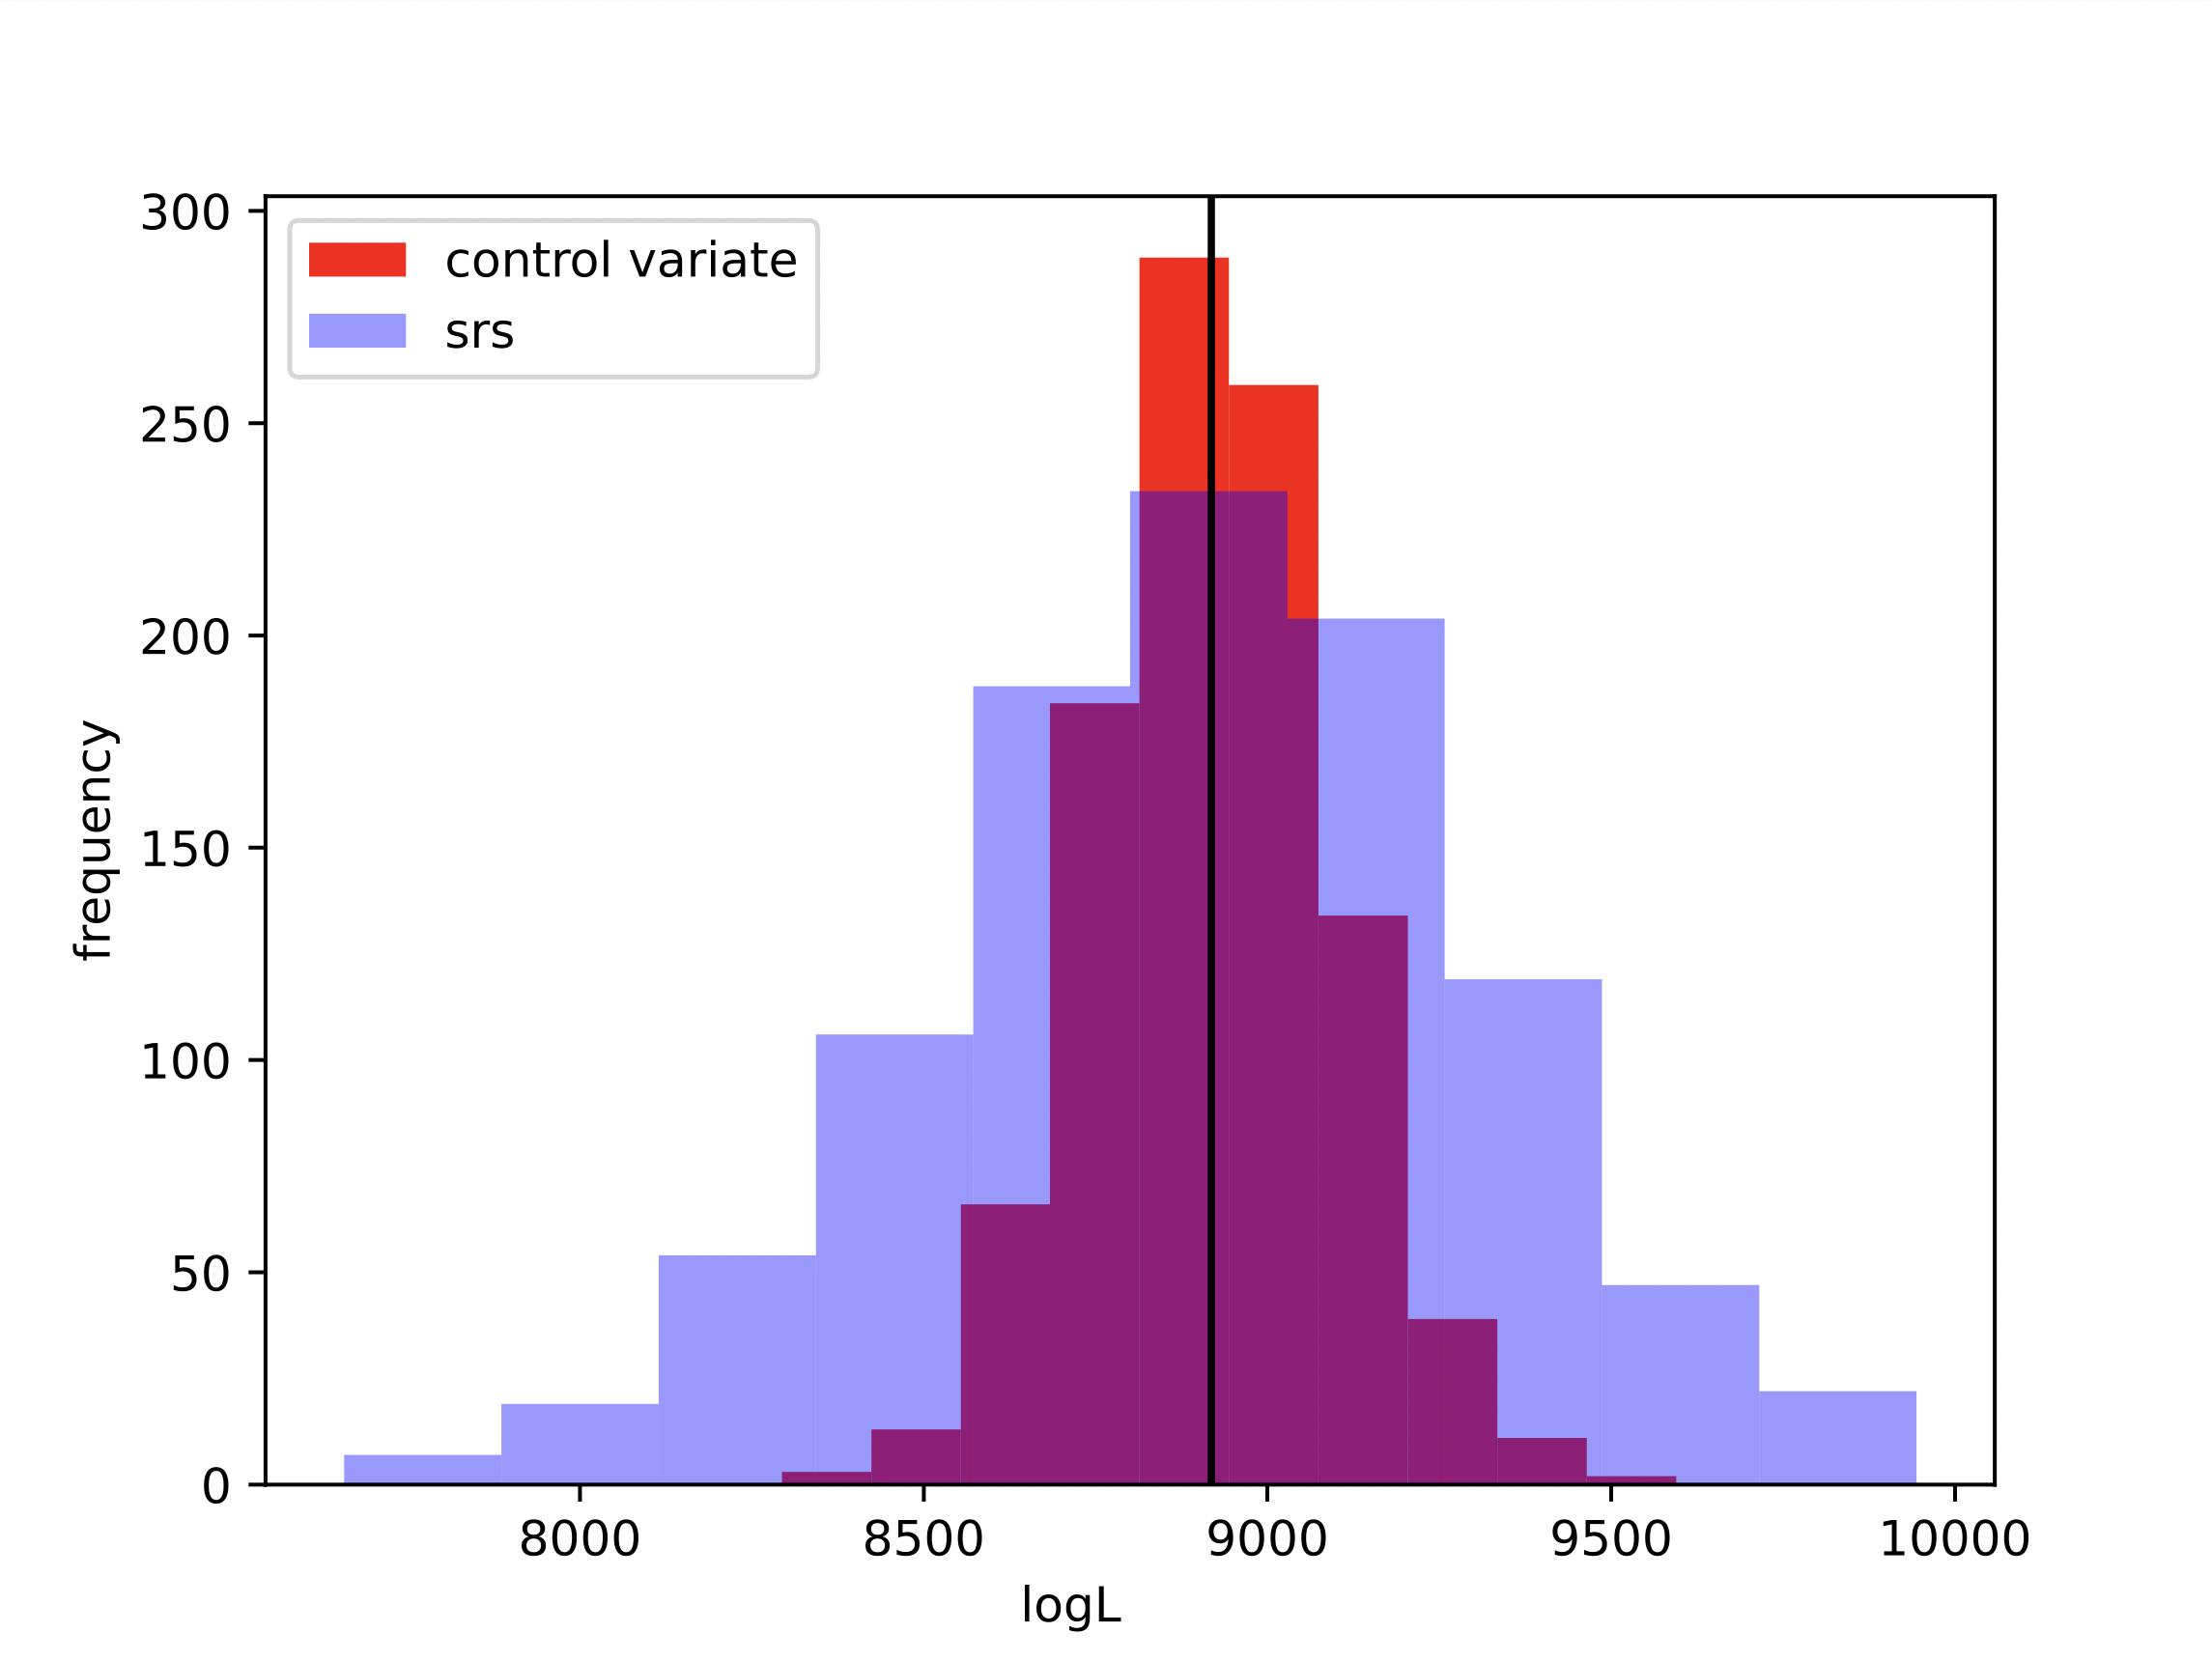
\includegraphics[width=1.0\textwidth]{Chapter3/Figs/regen3_29.png}
\caption{ The plotted histograms represent the total log-likelihood values for the third degree polynomial $f(x,\theta)$ mentioned above in \cref{eq:tertiary poly}. There are $100$ $\log L(\theta)$ samples plotted for both histogram plots. The $\theta$ chosen are the true values of the parameters of our model, namely $b=2$ and $c=1$, referring to \cref{eq:tertiary poly}. The black vertical line represents the true value of the total log-likelihood. The blue histogram represents the values estimated by the SRS method without control variates. The control variate subsampling method produces the red histogram. The control variate method is significantly superior to simple random sampling in these results. The standard deviation of the results given by the control variate method is $2.5$ times less than the simple random sampling.}
\label{fig:gggh}
\end{figure}

In this section the control variate subsampling method has been applied to a toy function, $f$. Now let us look into further detail regarding the computational costs of this method.


\subsection{Computational Costs}\label{sec:computational_costs}
In the Quiroz et al. paper~\cite{Quiroz_2018}, the computation costs of evaluating \cref{cvv} were quoted as
%
\begin{equation}
\mathrm{cost} = K \cdot c_{\bar{l}} + m \cdot c_{l}.
\end{equation}
Here  $c_{\bar{l}}$ is the computational cost of evaluating a control variate, $c_{l}$ is the cost of evaluating a single log-likelihood contribution, $m$ is the number of subsamples and $K$ is the number of cluster centres. Note, we only need to allocate the points to their respective clusters once, and evaluate the $(z_i-\bar{z_{k_i}})$ terms in \cref{cvv} once. We only need to do these once because this is at the data level, which is fixed--rather than the parameter level, which vary throughout the fit. This effectively renders only $K$ unique $\bar{l}$ terms to be evaluated for the whole dataset at each MCMC or nested sampling iteration.

Since $K \ll m,n$, this shows that the computational costs are roughly equivalent to SRS with a similar $m$--all while producing much more accurate results (Assuming $c_{\bar{l}} \approx c_{l}$ which is not unreasonable). In the common case of a Gaussian-distributed error on the response variable, the computational cost relationship is 
%
\begin{equation}
    c_{\bar{l}} \approx 7*c_{l}.
\end{equation}
%
This is since that $l(\bar{\textbf{z}}_{k_{i}},\theta)$ in \cref{eq:taylor} has $1$ independent sum; $\nabla_z l(\bar{\textbf{z}}_{k_{i}},\theta) \cdot (\textbf{z}_i-\bar{\textbf{z}}_{k_{i}})$ has $2$ sums since it is a vector dot product; and, finally, $\frac{1}{2}(\textbf{z}_i-\bar{\textbf{z}}_{k_{i}})^\intercal  \nabla_z \nabla_z l(\bar{\textbf{z}}_{k_{i}},\theta)(\textbf{z}_i-\bar{\textbf{z}}_{k_{i}})$ has $4$ independent sums, since it goes from a matrix to a scalar. For concreteness we shall be more explicit in what we mean by independent sums. When we say 4 separate sums for $\frac{1}{2}(\textbf{z}_i-\bar{\textbf{z}}_{k_{i}})^\intercal  \nabla_z \nabla_z l(\bar{\textbf{z}}_{k_{i}},\theta)(\textbf{z}_i-\bar{\textbf{z}}_{k_{i}})$ we mean that once we carry out this matrix multiplication there are 4 independent `numbers' that we have to sum up to get the value. These all add up to $7$ separate terms. This is in comparison with each log-likelihood only having $1$ separate term. Thus for the computational costs to align we had the constraint,
%
\begin{equation}
    K \cdot 7 + m_{\textrm{Control Variate}}= m_{\textrm{SRS}}.
\end{equation}
%
Here $m_{\textrm{Control Variate}}$ and $m_{\textrm{SRS}}$ are the $m$s used in the control variate and SRS methods respectively (refer to what we label $m$ in \cref{eq:fgf} and \cref{cvv} respectively). 



\subsection{Voronoi Cell Averaged Subsampling Comparison with Control Variate Subsampling}\label{sec:voronoi}


We have shown promising results suggesting that control variate subsampling may be better than SRS in some cases. However, for the purpose of this thesis we must also compare with results the Voronoi cell averaged subsampling technique used in \cite{Mihaylov_2020}. Doing so will support our main assertion in \Cref{ch:chapter4}: that our newly proposed control variate subsampling method will ideally improve the accuracy of the Bayesian analysis performed in the gravitational wave detection technique in the original paper \cite{Mihaylov_2020}. This paper uses the aforementioned Voronoi subsampling method for sampling likelihoods. Briefly, Voronoi cell averaged subsampling consists of clustering all the data points by the Voronoi cells--i.e.\ labelling them to the Voronoi cell that they are closest to in data-space--then, averaging over all the points in a Voronoi cell to get a Voronoi cell average. After this is performed, for every subsequent sample of the likelihood function, this average value average value of the data of a particular Voronoi cell is then used in place of every point that exists within the Voronoi cell. This evidently results in a deterministic likelihood. For further detail refer to \cite{Mihaylov_2020}.


Since Voronoi cell averaged subsampling is completely deterministic we cannot repeat the comparisons performed in \cref{fig:gggh} again to analyse its utility. It would not produce a histogram with a spread as seen in \cref{fig:gggh}, but rather a simple vertical line due to its deterministic nature. A better comparison would be of the accuracy of the resulting $\log Z$ values produced by each sampling method for the Bayesian analysis performed on the third degree polynomial `model' from \cref{eq:tertiary poly}. The evidence values were calculated by carrying out orthodox nested sampling--but in place of the usual likelihood we plugged a non-deterministic likelihood generated by one of the subsampling methods. For all three subsampling methods, SRS, Voronoi cell average subsampling, and control variate subsampling, we shall use `hyperparameters'--$n$, $m$ and/or $K$--which result in equivalent computational cost for all 3 sampling method runs, to produce a like-for-like comparison. The total number of data points used were $n=10,000$. The number of Voronoi cells was $300$ and similarly the subsample size $m$ for SRS was $300$ at each subsample. To get the equivalent computational cost for a control variate subsample we must set $k=22$ and $m=146$; where we used the computational cost calculations from the previous section.



\begin{table}[h!]
\begin{center}
\begin{tabular}{c|c}
Method                              & $\log Z \pm \sigma$ \\
\hline
Voronoi cell average subsampling    & $13,597 \pm 0.4$    \\
SRS                                 & $9,105 \pm 0.7$     \\
control variate subsampling         & $8,920 \pm 0.8$     \\
deterministic full dataset sampling & $8,850 \pm 0.4$    
\end{tabular}
\end{center}
\caption{Log-evidence values produced by the different subsampling methods\label{tab:subsampling}}
\end{table}

We can see that not only did control variate subsampling outperform the Voronoi subsampling method used in \cite{Mihaylov_2020}, but so did simple random subsampling. Control variate subsampling was by far the closest in producing the correct $\log Z$ value--which is labelled by ``deterministic full dataset sampling'' in \cref{tab:subsampling}. This yet again shows that, if we can get past the turmoil related to the unsuitability with non-determinism of the current nested sampling packages, we are far better off dealing in non-deterministic subsampling rather than deterministic. The reason papers in the literature, such as Ref \cite{Mihaylov_2020}, widely avoided non-determinism was not because it is less accurate. Rather they avoided it because none of the widely used nested sampling packages could cope with non-determinism. Thus, in the next section we show how to implement non-deterministic log-likelihoods into nested sampling in the following section.

Note that the \cref{tab:subsampling} shows favourable results for control variate subsampling over the Voronoi averaging method. This is true even though the particular model and data we were dealing with, were as favourable as it gets for Voronoi averaged subsampling. Even with all the advantages of a suitable problem, Voronoi subsampling still significantly underperformed control variate subsampling. The reason for this being an advantageous problem for Voronoi subsampling is that the variation of the data spanned within a particular Voronoi cell is minute. The range spanned by our data is $x=[-1,1]$, and within this small region are packed $300$ Voronoi cells. Another requirement given in \cite{Mihaylov_2020} for the Voronoi subsampling method to be maximally accurate is that the error associated with each data point has to be independent from the others. This requirement is built into our toy model. Yet, the control variate subsampling still produced more favourable results. Note, as well, that our subsamples $m$ were only on a scale of roughly $30 \times$ smaller than the total dataset $n$. 





\section{Which Nested Sampling Algorithm is Best Suited to Tackle Non-Determinism?}\label{sec:nondet}

In exploring how to accurately implement nested sampling on non-deterministic likelihoods we tried the implementation of multiple versions of nested sampling algorithms. It is not clear to what extent the nested sampling meta-algorithm is valid for non-deterministic likelihoods. However, we made some preliminary investigations that are the subject of ongoing research.


\subsection{How We Simulated Non-Determinism}
The way we generated ``non-deterministic'' likelihoods was by first generating the dataset of $\{x_i,y_i\}$. The model for $y$ that we are trying to test our model that was
\begin{equation}
F(x)= bx+c.
\end{equation}
This function acts as our ``theory model''--analogous to an equation of a physical theory we may be testing against data. It has two parameters that we seek to find out the true value of--$\theta = [b,c]$. $\{x_i\}$, was generated by drawing them uniformly between $-1$ and $1$. Then by taking a randomly selected subset of this dataset $\{x_i\}$ and feeding it again into the function above, $F(x_i)$, we generated the subsample that generates a non-deterministic log-likelihood:
%
\begin{equation}
    \log L = \frac{n}{m}\sum_j^m -\frac{\log (2\pi\sigma^2)}{2} - \frac{ (y_j - F(x_j)^2}{2\sigma^2}.
\end{equation}
%
Here, $n$ is the size of the full raw dataset, $m$ is the size of the selected subsample of the dataset, $j$ is the dummy variable we sum over. For the non-deterministic runs of nested sampling, whenever we sample the log-likelihood we have a newly randomly selected subset $x = \{ x_{k_0}, x_{k_1},...,x_{k_m}\}$ of the full dataset $x= \{ x_0,x_1,...,x_n \}$ to get a dataset of $F(x_i)$. At each call of the log-likelihood function in the code by nested sampling, such a new sub-dataset is used to generate the non-deterministic log-likelihood. Depending on which random subset is sampled from the full raw dataset, the same parameters choice, $\theta$, may yield different log-likelihood values.



\subsection{Bayesian Evidence of Non-deterministic Likelihood}


\begin{figure} 
\centering    
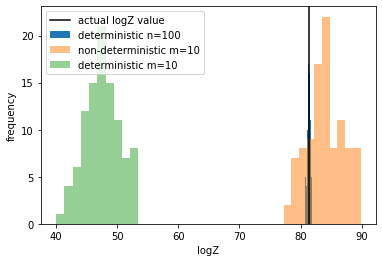
\includegraphics[width=1.0\textwidth]{Figure 2022-09-02 221530}
\caption[Orthodox]{Histograms of log Z values from Metropolis Hastings nested sampling. The deterministic likelihood using the full dataset produced the most ideal results. The non-deterministic likelihood produced evidence values that were less accurate but contained the true value within their error margin. However, the deterministic likelihood that did not use the full dataset, represented by the green histogram, did not even contain the correct values within the distribution. There are 100 $\log Z$ values plotted in each histogram.}
\label{fig:logZ2}
\end{figure}

\begin{figure} 
\centering    
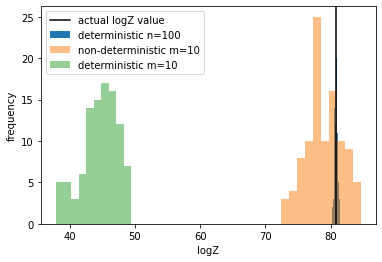
\includegraphics[width=1.0\textwidth]{logz_hist_orthodox1}
\caption{Histograms of $\log Z$ values from orthodox nested sampling. Again, the deterministic likelihood using the full dataset produced the most ideal results. The non-deterministic likelihood produced evidence values that were less accurate but contained the true value within their error margin. However, the deterministic likelihood that did not use the full dataset, represented by the green histogram, did not even contain the correct values within the distribution. The exact true value of $\log Z$ is plotted for reference as well as the black vertical line. There are 100 $\log Z$ values plotted in each histogram. }
\label{fig:logZ11}
\end{figure}


All 100 of the $\log Z$ values in \cref{fig:logZ11} are derived from a single set of $\log L$ values. This is to be as true to the circumstances we would find in the real world where the computationally limiting factor is sampling the $\log L$ values. Simulating the corresponding sets of $\log X$ values to go along with this one set of $\log L$ values is computationally trivial in comparison, thus these 100 $\log Z$ values come from one set of $\log L$ values paired with 100 sets of simulated $\log X$ values. We can see that the deterministic subsample is far off mark, as expected. The non-deterministic subsample run fares much better. As expected the variance of the log-evidence values from the full dataset is far smaller than the from the subsamples.


The Metropolis Hastings nested sampling works nearly the same as orthodox nested sampling except with an altered mechanism of suggesting a new live point at each iteration. Instead of completely randomly selecting new points from the same domain until one satisfies acceptance criteria, we start with an already acceptable live point and take a `random walk' starting from there. In our version of Metropolis Hastings nested sampling, we propose a new point by: identifying the live point corresponding to the lowest likelihood, taking a number of steps as increments in the parameter space, and only accepting a proposed step if it has gone in a direction of increasing log-likelihood in parameter space. The step looks like this:
%
\begin{equation}
\theta_\mathrm{old}=\theta_{\mathrm{new}}+\epsilon.    
\end{equation}
%
Here, $\epsilon$ is selected as a random variable vector distributed as a normal distribution with mean zero and covariance equal to the covariance of the parameter space dataset of current live points.

We believe that Metropolis Hastings is inherently better suited to deal with non-determinism due to its step by step walk which allows it to stay within the allowed iso-likelihood contours even in the midst of large log-likelihood function uncertainty. This is supported by our preliminary testing, in which we found Metropolis Hastings nested sampling to converge quicker than orthodox nested sampling while achieving a similar level of accuracy.



\subsection{Stopping Criteria}
Non-deterministic likelihoods require significant care into the choice of a stopping criteriion. The stopping criterion that we implemented was that if the mass contributions, $ Z_n = L_nw_n$, to of the cumulative evidence up until the latest iteration, $ Z = \sum_i^n L_iw_i$, was smaller than some given tolerance,
\begin{equation}
\frac{ Z_{n}}{ Z}< \epsilon_{\mathrm{tol}}
\end{equation}
 for five consecutive nested sampling steps, then the algorithm would terminate. The idea behind this is that continuing the algorithm will experience diminishing returns after some point such that the contributions to the evidence are consistently below some threshold that we deem appropriate. The reason we require that this happens 5 times consecutively is that due to the probabilistic nature of nested sampling, we may erroneously encounter a small increment in evidence mass. This doesn't necessarily mean that the actual posterior mass increments are going to be small then-on, but if it happens 5 times in a row then it likely was not due to a chance event.

 Our stopping criterion is somewhat of a proxy for that which is generally used in the nested sampling literature, the approximate remaining evidence by total accrued evidence. \texttt{MultiNest} and \texttt{PolyChord} both use estimators of this and set a tolerance for the fraction of estimated remaining posterior mass. \texttt{PolyChord} has the break condition:
%
 \begin{equation}
\bar{L}(1-X_i)/Z=\Delta Z/Z<\mathrm{tol},
 \end{equation}
%
 where $\bar{L}$ is the average likelihood taken from all the samples. We found this breaking criterion to be perhaps too stringent in the case of non-deterministic likelihoods. We find that significant noisiness in the likelihood may cause uncharacteristic oscillations in the accumulated evidence at each iteration which would prevent termination of nested sampling indefinitely. Perhaps this is among the reasons \texttt{MultiNest} and \texttt{PolyChord} struggle. However this is not a conclusive remark and more work needs to be done on this. Trying to counter this one may reduce the tolerance to a significant degree. However, when the magnitude of non-determinism becomes too large we may also find that we may make increments in the evidence that are uncharacteristically low, causing premature termination of the algorithm. In such circumstances we chose to put a hard constraint of total number of nested sampling algorithm iterations before algorithm termination. Trial and error may be used to determine an appropriate value for the number of iterations before termination.

 \subsection{Summary of Compatibility of Various Nested Sampling Algorithms with Non-deterministic Likelihoods}

 A summary of our preliminary explorations:



\begin{enumerate}
    \item \texttt{PolyChord} is a nested sampling algorithm that uses slice sampling. Slice sampling consists of sampling within a likelihood bound using an already existing live point and a guess of the bound size. This sampling method completely failed to converge. \cite{Handley_2015} This is because slice sampling assumes a deterministic likelihood, and therefore would never work. Slices regularly fail to to terminate under a likelihood that fluctuates and changes the bounds of a slice.

     \item Our own orthodox nested sampling that we coded from scratch converged, as can be seen in \cref{fig:logZ11}. Orthodox nested sampling uses `brute force' rejection sampling from the unit hypercube until a point is found within it. This is therefore not generally scalable but for the small problems we consider here acts as a good point of reference. 
    \item \texttt{MultiNest} uses rejection sampling from the unit hypercube as well. Its rejection sampling quickly breaks down as soon as the non-determinism becomes significant and, thus, fails to converge~\cite{Feroz_2009}. As alluded in the section above, we believe that this may be due to their choice of stopping criterion.
   
    \item Our own Metropolis Hastings nested sampling coded from scratch, which used a random walk from an already existing live point to sample new points. Our algorithm consistently converged. This is shown in \cref{fig:logZ2}. \cite{doi:10.1080/00031305.1995.10476177}
\end{enumerate}

\section{Conclusions}


Our main conclusion is that all of our results show non-deterministic subsampling performs favourably over deterministic subsampling. Theoretically this should be true given that the number of times the subsamples are drawn is sufficient, which we believe is often the case for MCMC and nested sampling. Several results across this chapter suggest this. Our major contribution is not only in introducing to the astronomy scientific community an improvement to SRS, in efficient subsampling through control variates, but also in showing how simple non-deterministic likelihoods can actually be made viable for nested sampling. To the best of our knowledge, this incorporation of non-deterministic likelihoods in nested sampling has not been examined in the astrostatistics literature before this thesis. Regarding control variate subsampling, the control variates, from \cref{eq:taylor}, encompass the information encoded in the global landscape of the log-likelihood over all of data-space. The control variate subsampling scheme also accounts for local effects and thus has the same local precision benefits as SRS, since it not only has a Taylor series spanning the whole data space, but also local subsamples as in SRS. This contributes towards making control variate subsampling a robust method. The Taylor expansion terms--first sum in \cref{cvv}--give a picture of the general macro-structure and information encoded within the log-likelihood manifold over the whole of the data space. On top of this, the subsampling terms--the second sum in \cref{cvv}--give a localised view of the smaller scale structures. The accuracy and precision of control variate subsampling as compared to SRS grows as the ratio $n/m$ grows. So, for big data, such as cosmological datasets, stock market data, large language model training datasets etc., control variate subsampling becomes increasingly favourable as the task becomes more data-intensive.

